\documentclass[letWterpaper,10pt,titlepage]{article}

\usepackage{graphicx}
\usepackage{amssymb}
\usepackage{amsmath}
\usepackage{amsthm}
\usepackage{alltt}
\usepackage{float}
\usepackage{color}
\usepackage{url}
\usepackage{balance}
\usepackage[TABBOTCAP, tight]{subfigure}
\usepackage{enumitem}
\usepackage{pstricks, pst-node}
\usepackage{geometry}
\geometry{textheight=10in, textwidth=7.5in}
\newcommand{\cred}[1]{{\color{red}#1}}
\newcommand{\cblue}[1]{{\color{blue}#1}}
\usepackage{hyperref}
\usepackage{textcomp}
\usepackage{listings}

%% The following metadata will show up in the PDF properties
\hypersetup{
  colorlinks = true,
  urlcolor = black,
  pdfkeywords = {cs325 ``Analysis of Algorithms'' subarray sum},
  pdftitle = {CS325 Project 1},
  pdfsubject = {CS325 Project 1},
  pdfpagemode = UseNone
}

\definecolor{comment}{rgb}{0, 0.6, 0}

\lstset{
    belowcaptionskip=1\baselineskip,
    breaklines=true,
    frame=single,
    xleftmargin=\parindent,
    language=Python,
    showstringspaces=false,
    basicstyle=\footnotesize\ttfamily,
    identifierstyle=\color{blue},
    stringstyle=\color{orange},
    commentstyle=\color{comment},
}

\parindent = 0.0 in
\parskip = 0.2 in


\begin{document}

\title{CS 325 Project 2: Coin Change}
\author{Project Group 25:\\Jonathon Moore\\Jaden Diefenbaugh\\Kenneth Hafdahl}
\maketitle

\section{Dynamic Programming Table Justification}
The dynamic programming table for changedp is allocated as an empty list with a size of $amount + 1$. This size allows each value from $0$ to $amount$ to be represented and stored for later use. The values in table are populated as recursive calls to changedp are made. The function checks if the listing for the corresponding amount is empty. If it is, the amount is calculated. Otherwise, it returns the value that was previously stored in the table. I think that this is a valid way to fill the table since values are calculated only once during the first time they are needed.

\section{Pseudocode}

\subsection{changeslow}

\begin{lstlisting}
# V is array of coin values and A is desired change amount
def changeslow(V, A):
    # coin counts with indices corresponding to V
    C = zeroed array that is size of V
    # Total number of coins
    T = 0
    if A in V:
       C[A index] = 1
       T = 1
    else:
        for i in from 1 .. A:
            res1 = changeslow(V, i)
            res2 = changeslow(V, A - i)
            if res1 + res2 total < T or T == 0:
               C = res1 + res2 arrays
               T = res1 + res2 totals
    return (C, T)
\end{lstlisting}

\subsection{changegreedy}

\begin{lstlisting}
# V is array of coin values and A is desired change amount
def changegreedy(V, A):
    k = len(V) - 1
    while k >= 0:
        if (V[k] == S):
            return [V[k]]
        if (V[k] > S):
            k -= 1;
        if (V[k] < S):
            sum2 = S - V[k]
            coins2 = V[:k + 1]
            return [V[k]] + algorithm2(sum2, coins2)
\end{lstlisting}

\subsection{changedp}

\begin{lstlisting}
# V is array of coin values and A is desired change amount
#table of minimum coin combinations for a given set of coins
coinTable = []
def changedp(coinValues, amount):
    if amount not in cointable:
        if there is an amount-cent coin:
            populate coinTable[amount] with single coin of size amount
        else:
            find the minimum number of coins needed to make i cents
            find the minimum number of coins needed to make amount - i cents
            choose the i and (amount-i) that minimizes sum and populate coinTable[amount]
    return coinTable[amount]
\end{lstlisting}

\section{Proof}
By definition $T[0]=0$.
Let's assume that $T[v]$ will always produce a list with the minimum number of coins. This also means that all $T[1..v]$ evaluates to the smallest amount of coins, as they have already been completed to reach $T[v]$. We need to show that $T[v+1]$ will also produce a minimum set of coins as an answer. $T[v+1]$ will look through all coins with values of $V[i]$ less than or equal to $v+1$. It will compare the number of coins for solutions $T[(v+1)-V[i]]$ for every value of $V[i]$ that is less than or equal to $v$. From here, there are one of two possibilities:

\begin{enumerate}
\item There exists a value of $V[i]$ equal to $(v+1)$ so that $(v+1)-V[i]=0$. $T[0] = 0$, so that $T[v+1]=T[0]+1$.

\item There does not exist a value $V[i]$ equal to $(v+1)$. Here we check every value $V[i]$ that is less than $(v+1)$ and subtract for that coin's value $(v+1)$, and then compare the remaining amount $T[v+1-V[i]]$ against the solution table we already have established. Because we have produced the solution in the dynamic manner, we have already computed all minimum solutions from $T[0..v]$. and we know that $(v+1-V[i])$ is a positive integer that is less than $(v+1)$. We then retrieve all solutions $T[v+1-V[i]]$ and select the one with the smallest coin set, adding $V[i]$ to its coin set to get the answer for $T[v+1]$. By our hypothesis all values of $T[1..v]$ will already produce the smallest coin set, and since $v+1-V[i]$ for any $V[i]$ is going to be between 1 and $v$, that will give us the optimal solution, which we then add 1 to account for the coin $V[i]$.
\end{enumerate}

\section{V=[1,5,10,25,50] A=[2010,2015,2020,...,2200]}
\begin{figure}[!ht]
    \centering
    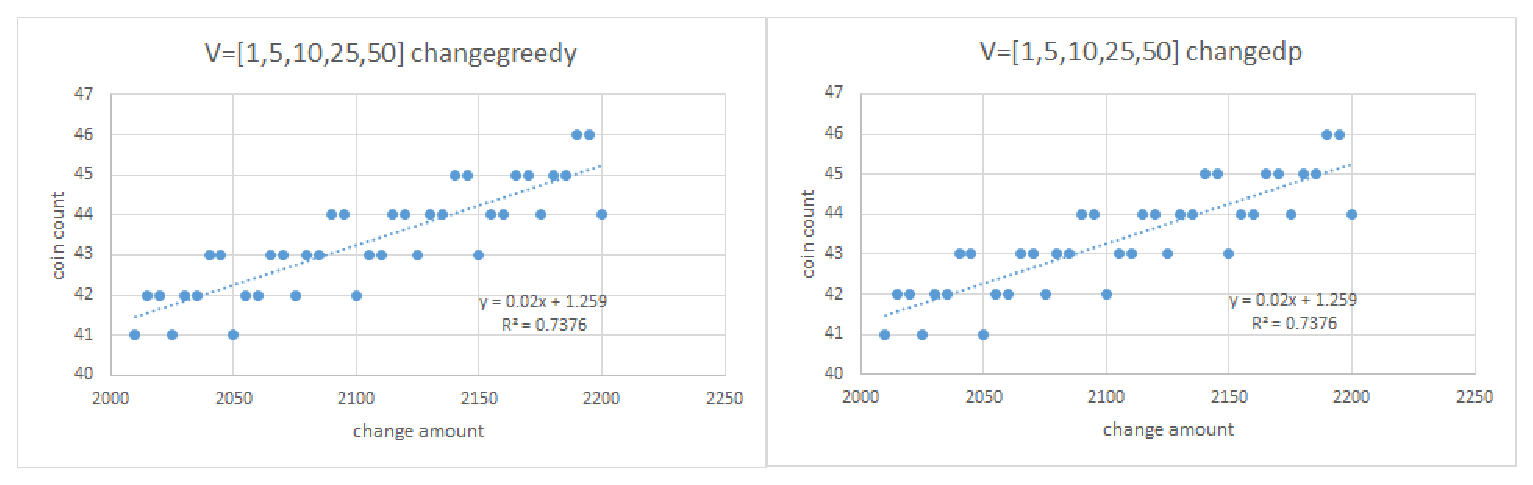
\includegraphics[width=0.75\textwidth]{./p4.eps}
\end{figure}
The resulting coin counts for the greedy and dynamic programming implementations are exactly the same for this given coin set. The trend line appears to be linear.

\section{$V_1$=[1,2,6,12,24,48,60] $V_2$=[1,6,13,37,150]}
\begin{figure}[!ht]
    \centering
    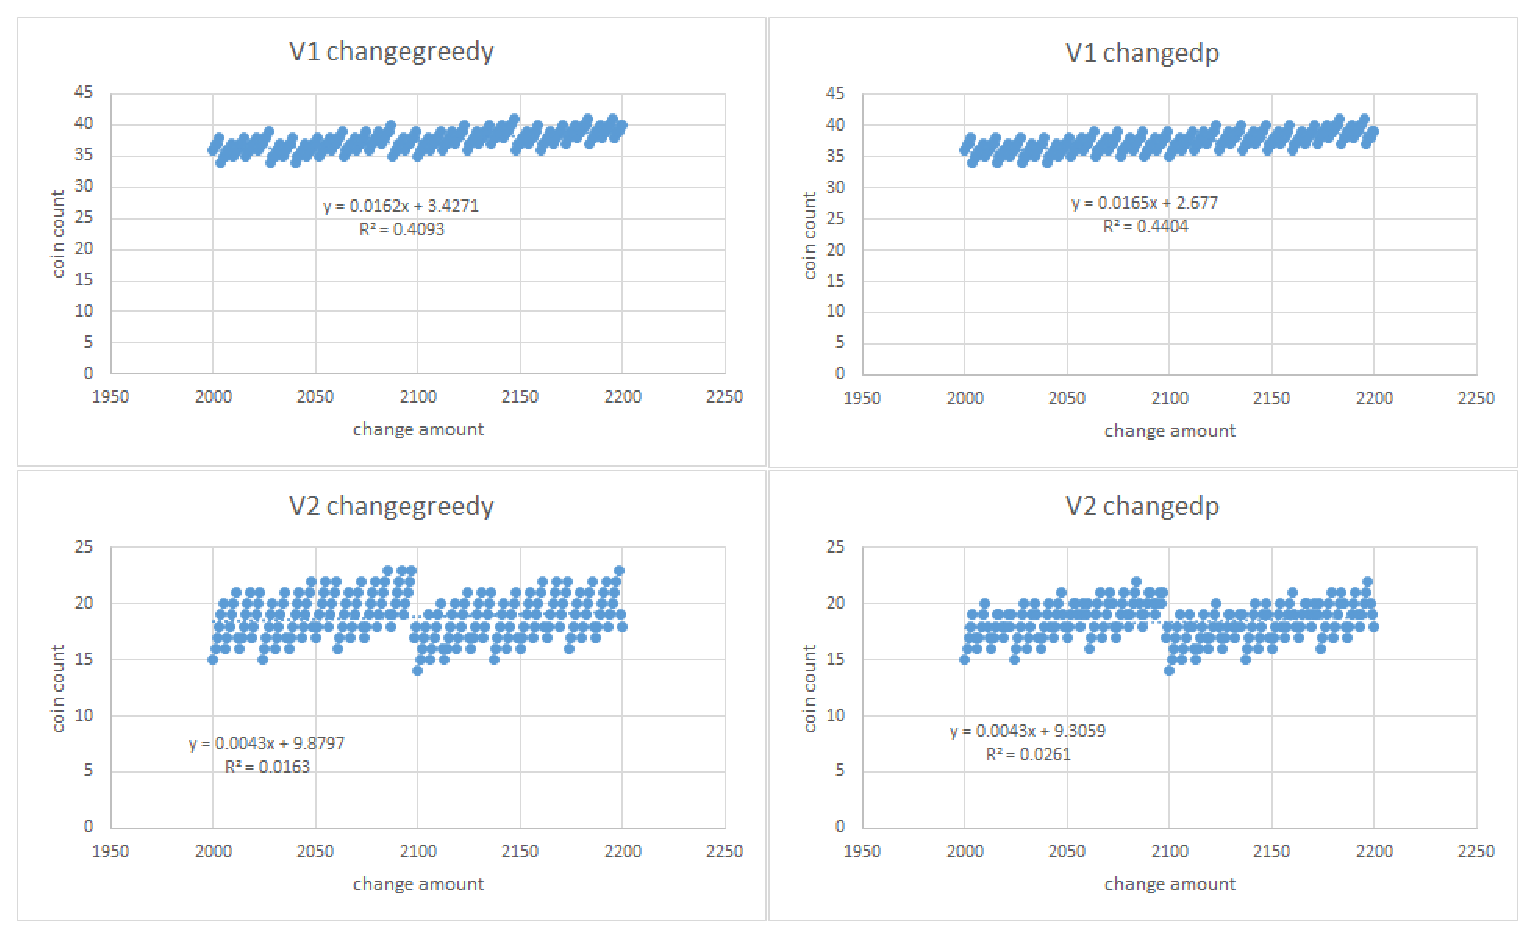
\includegraphics[width=0.75\textwidth]{./p5.eps}
\end{figure}
The groupings for changedp were tighter than those found in changegreedy. However, the rate in which the coin count increased was nearly identical for both algorithms. In most cases, the coin counts matched. The largest difference between the two sets was three coins. Both sets seem to follow a roughly linear trendline.

\section{V=[1,2,6,12,24,48,60] A=[1,6,13,37,150]}
\begin{figure}[!ht]
    \centering
    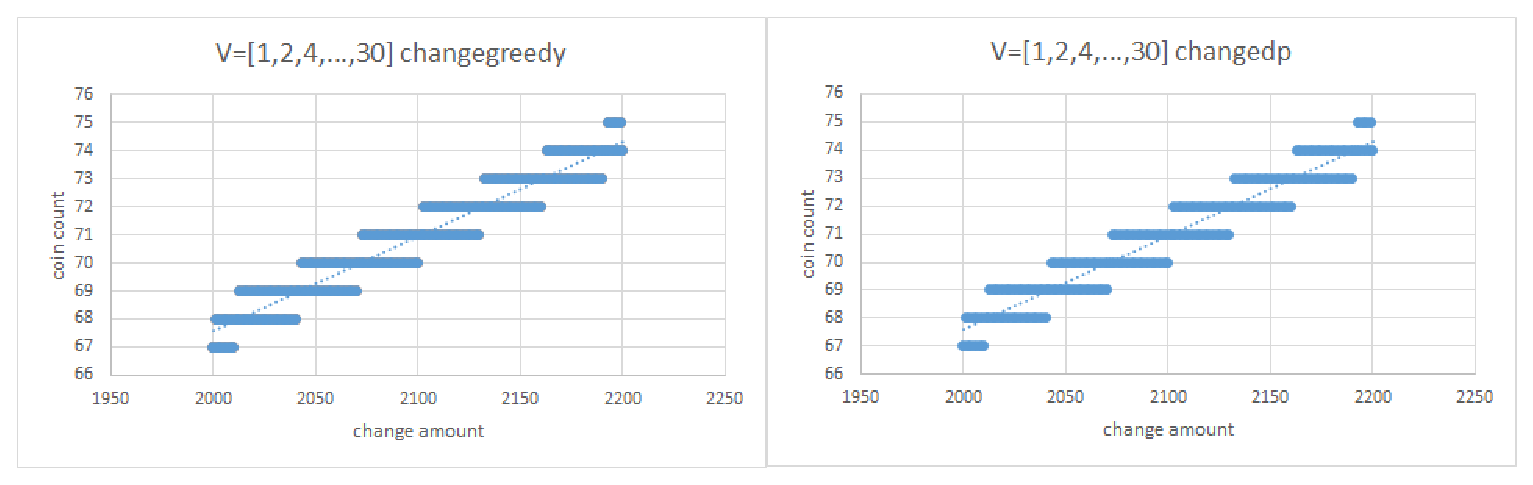
\includegraphics[width=0.75\textwidth]{./p6.eps}
\end{figure}
The coin coin counts for this particular coin set resulted in identical sets between the greedy algorithm and dynamic programming algorithm. It appears that coin sets that have values that evenly divide each other play nice with the greedy algorithm.

\end{document}
